xtick={1,2,3},xticklabels={1 lane,2 lanes,3 lanes},
ylabel={Aggregate completion throughput (tok/s)},
axis lines*=left,
major grid style={dotted},ymajorgrids=true,
error bars/y dir=both,error bars/y explicit,
nodes near coords,nodes near coords align={vertical},
every node near coord/.append style={font=\scriptsize},
]
\addplot+[draw=black,fill=gray!25,error bars/y dir=both,error bars/y explicit]
coordinates {(1,71.45) +- (0,1.12) (2,137.57) +- (0,2.19) (3,191.75) +- (0,7.24)};
\end{axis}
\end{tikzpicture}
\caption{Common-wall independent-request scaling (mean $\pm$ SD, $n=5$). The third point is measured on an x8/x8/x4 topology; the experiment does not separate PCIe-width effects from other shared-resource contention.}
\label{fig:scaling}
\end{figure}

The experiment establishes useful request-level scaling on this particular asymmetric topology, but it does not identify the source of the remaining 10.5\% loss. PCIe width, CPU/core placement, DRAM traffic, thermal state, and other shared resources are confounded. We therefore treat 89.5\% as an operating-point measurement rather than evidence for a particular contention mechanism.

\subsection{RQ2: Does shared backing eliminate replica RAM duplication?}
The two-engine private control measures 95.3~GiB PSS, while shared backing measures 52.1~GiB, a reduction of 43.2~GiB or 45.4\% (Figure~\ref{fig:memory}). The shared arena appears as the same \texttt{rw-s} \texttt{/dev/shm} mapping in both engines. The 49,116,200~KiB arena mapping is accounted as \texttt{Shared\_Dirty}, with \texttt{Private\_Dirty=0}. This is direct OS-level evidence of physical sharing rather than an inference from virtual address size or RSS.

\begin{figure}[t]
\centering
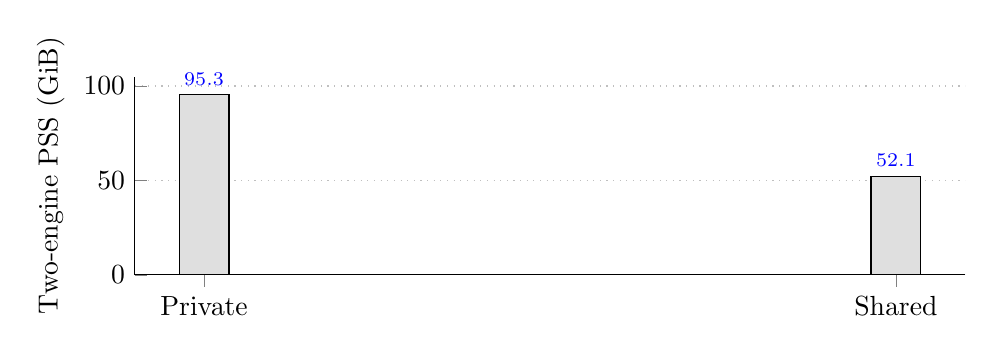
\begin{tikzpicture}
\begin{axis}[
width=\columnwidth,height=4.1cm,
ybar,bar width=18pt,ymin=0,ymax=105,
xtick=data,xticklabels={Private,Shared},
ylabel={Two-engine PSS (GiB)},
axis lines*=left,ymajorgrids=true,major grid style={dotted},
nodes near coords,every node near coord/.append style={font=\scriptsize},
]
\addplot+[draw=black,fill=gray!25] coordinates {(1,95.3) (2,52.1)};
\end{axis}
\end{tikzpicture}
\caption{Physical-memory ablation. Sharing one host expert arena reduces two-engine PSS by 43.2~GiB (45.4\%).}
\label{fig:memory}
\end{figure}

The measured PSS reduction (43.2~GiB) is smaller than the 46.8~GiB shared mapping size by about 3.6~GiB. The benchmark snapshots also differ in host-global used swap: 9.44~GiB for the private arm and 5.70~GiB for the shared arm. Numerically, adding those global swap counters gives 104.74 versus 57.79~GiB, a 46.95~GiB difference close to the arena size. However, the swap counter covers the whole host, not just the two engine processes, so this near-match is suggestive rather than proof that the arena alone caused the swap delta. We therefore keep PSS as the primary directly attributable process metric and disclose the swap observation separately.

